\chapter{System Description} % Main chapter title

\label{sysdes} % For referencing the chapter elsewhere, use \ref{Chapter1} 

\lhead{Chapter 4. \emph{System Description}} % This is for the header on each page - perhaps a 

\section{Overview}
\label{sect:sysdesover}

As mentioned in Section \ref{subsec:knn}, before applying a nearest neighbors algorithm, one must normalize dimensions proportional to their relevance.  Conventionally, if the relevance of a dimension or a set of dimensions were to be changed, one must perform a linear transformation on the every single point in the search space.  When using an index type described in Section \ref{sec:ann}, this linear transformation requires a total reconstruction of the index for optimal nearest neighbors search performace, as the distance between all pairs of points in the index is now different.

The goal of this system is to support queries of dynamic dimension relevance in low dimensional spaces.  Dynamic dimension relevance means that requester of a given query must provide both a search point, and the relevance of each dimension in the query.  The system will then compute the ANNs using a modified Euclidean distance metric in which the distance in each dimension is weighted proportionately to the relevance.  This metric is described formally in Section \ref{subsec:dimrel}.

\subsection{Normalization}
\label{subsec:normalization}

Each dimension in the vector space representation of a dataset must be normalized to ensure that each dimension is initially weighted equally.  The normalization scheme used performs a linear transform to set the mininum value of a dimension to zero and the maximum value to one.  After finding the minimum and maximum of each dimension, one must normalize every dimension of every point following Equation \ref{eq:normd}.

\begin{equation}
\label{eq:normd}
d_{normalized} = \dfrac{d-d_{min}}{ d_{max} - d_{min} }
\end{equation}

This normalization technique is ideal for datasets which follow a relatively uniform distribution.  However, the presence of outliers could greatly skew this normalization scheme.  An alternative normalization strategy for these cases is to normalize the mean of each dimension to zero, and the standard deviation to one.  This can be achieved by following the linear transformation outlined in Equation \ref{eq:normd2}.  This procedure is equivalent to finding the standard score or z-score of each dimension \citep{cheadle2003analysis}.

\begin{equation}
\label{eq:normd2}
d_{normalized} = \dfrac{d-d_{mean}}{ d_{stdev} }
\end{equation}

\subsection{Dimension Relevance}
\label{subsec:dimrel}

After normalization described in section \ref{subsec:normalization}, each dimension in the dataset is said to have equal relevance, and would have an equivalent contributribution to a standard Euclidean distance.  As described in section \ref{sect:sysdesover} each query requires both a search point, and a dimension relevance vector (DRV).  The DRV must contain the same number of dimensions as all points in a dataset.  Each element in the DRV specifies a weight for a single dimension.  The DRV is then normalized to have a sum of one.  Using the DRV, v, and two D-dimensional points x and y, the modified Euclidean distance metric is shown in Equation \ref{eq:eucmod}.

\begin{equation}
\label{eq:eucmod}
distance = \sqrt{\sum\limits_{i=1}^D ((x_i - y_i) \times v_i \times D)^2)} \\
\end{equation}

For the case in which all dimensions are weighted equally, each element is $v_i=1/D$.  Thus, in this special case, the standard Euclidean distance is computed.  This distance metric is also equivalent to transforming each dimension via multiplying by $v_i \times D$, and computing the standard Euclidean distance.  By using this modified metric instead, this transformation does not need to be explicitly performed but is inherent in the distance calculation.  It should also be noted that for computational purpose one can disclude the multiplication by D, as this can factor out of the distance metric as a constant.  D was included such that this distance would better conceptually match the standard Euclidean distance.

\subsection{Motivation for k-d Trees}
\label{sec:kdtreemotiv}

We aim to tackle the the challenge of creating an ANN index which performs well when DRVs are specified at query time, and allows for queries of different quality requirements.  We opted to base our index on k-d trees for a variety of different reasons.  Graph indices, as described in Section \ref{sec:graphind} have a high offline construction cost, and compute the KNN of each node at construction time.  This makes them poorly suited to adapt to a changing distance metric.  Hash based indexes, described in Section \ref{sec:hashind} also have some downsides.  Generally, the hash functions used act as quantizers and aren't tied directly to dimensions in a vector space.  Additionally, the accuracy of hash based indexes is tied to the number of hash functions, and the amount of buckets of each.  As such this quality cannot be changed at query time.

Tree based indexes, described in Section\ref{sec:treeind} tend to be the most memory efficient in low dimensional spaces.  Additionally, the partitioning of tree indexes is inherentaly tied to the vector space representation.  A specific advantage of k-d trees, described in \ref{sec:kdtree} is that they are guaranteed to be linear in size, and splits can only occur orthogonal to a dimension.

\subsection{Split Dimension Determination Heuristics}
\label{section:splitdim}

A common heuristic for determining the split dimension on k-d tree indexes is spatial median splitting (SMS) \citep{zhou2008real,wald2006building}.  SMS always selects the longest dimensions as the one to split on.  The motivation for this technique is that each hyperrectangle should be as close to a cuboid as possible.  In doing so, the check of whether or not a ball of radius R around a point intersects with an enclosing hyperplane is more likely to result in no intersection.  When no intersection occurs, the k-d tree search algorithm described in Section \ref{sec:kdquery}, can eliminate a subtree without searching it.  It is important to note that k-d trees can still function, even if the partitions are not square.  However, because of the inability to prune subtrees as effectively, ANN searches will not be as efficient, and the quality of the result set under the constraint of a fixed number of searches will suffer.  It is also important to note that on a vector space in which each dimension has been normalized, selecting a random dimension to split on with equal probability accomplishes a similar effect to SMS.  On average, regions will tend to be close to cuboids. The advantage of this method is less offline computation in index construction and more variety in trees.  This additional variety is advantageous when searching multiple trees \citep{flann_pami_2014}.

When applying dimension weights via a DRV to a k-d tree search, the distance metric acts on a transformed space.  As such, if the split dimension is selected with SMS or randomly with equal probability on each dimension, the regions would no longer be cuboids on average.  Two different possible heuristics are applied to combat this.  The first is split probability matching (SPM).  The goal of this heuristic is to adjust the probability of splitting on each dimension to account for the fact that in the transformed space the dimensions are no longer normalized to the same weight.  Therefore, by selecting split dimensions with probabilities equal to the weight of each dimension, the regions will tend to approach a cuboid shape in the transformed space.  The second heuristic is weighted spatial median splitting (WSMS).  WSMS is performed the same way as SMS, however the distance between the maximum and minimum of dimension is multiplied by the dimension weight from the DRV.  Thus, this technique is equivalent to SMS on the transformed vector space.

\subsection{Initial Tests}
\label{sec:inittest}

The dataset used for our tests included 100,000 8 dimensional points, in which the value for each dimension is pulled from U(0,1).  100 different randomly generated DRVs were generated via applying U(0,1) in each dimension and normalizing to a sum of one.  10 query points were generated for each DRV following the same procedure as the generation of the dataset.  Thus, this test consists of 1000 queries on each index type.  For this test, K was set to 50, while the max number of nodes searched was set to 500.

Initially two k-d trees were generated.  One used SMS as its split dimension selection method, while the other selected randomly.  Additionally, two forests of three trees were generated. In the first, each tree used SMS to selected split dimensions, while in the other split dimensions were selected randomly.  For each of the generated DRVs, four new indexes were created.  A tree using WSMS, a tree using SPM, a forest of 3 trees using WSMS on each, and a forest of three trees using SPM on each.

A standard linear search was applied using the modified distance metric to determine the correct top K for each DRV and query point.  An ANN query was then performed using the eight different indexes (four of which are the same across all query points, while four were initialized using the seed DRV for each of the 100 seed DRVs).  The evaluation metric used is mean percent distance gain (MPDG).  The average distance of each set of K elements was calculated.  Then, using Equation \ref{eq:evalmetric} the average distance in each ANN set was compared to that of the linear search.  A gain in this average distance represents a lower quality result.

\begin{equation}
\label{eq:evalmetric}
MPDG = average\_distance_{index} / average\_distance_{linear} - 1 \\
\end{equation}

Figure \ref{fig:drvmatching} displays the results of these initial tests.  A single k-d tree using WSMS had the highest performance.  Spatial median splitting and its variant tended to perform better than the randomized methods, and single trees performed better than forests.  Figure \ref{fig:drv_varying_points}, shows a similar test with a varying number of points searched.  This figure however only includes the first results for a standard k-d tree using SMS and the variant using WSMS.  From this plot it can be seen that WSMS has significantly better performance with a low number of points searched, and eventually both SMS and WSMS converge to very accurate results given enough searching.  Another perspective which can be made from this plot is that under the constraint of a minimum quality, for any quality chosen, WSMS will return the result significantly faster.  For example, if a MPDG of .15 is required, WSMS would reach that level of quality approximately three times faster.  Thus, from these plots it is clear that both of these heuristics have the potential for better results.  Further evaluation is discussed in Chapter \ref{results} to determine scenarios in which both of these heuristics are most effective.

\begin{figure}[h]
\begin{center}
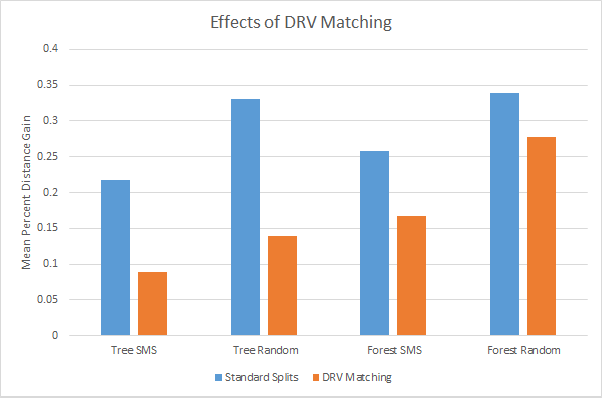
\includegraphics[width=\textwidth]{Figures/sysdesc_drvmatching}
\end{center}
\caption{Initial tests of DRV matching heuristics}
\label{fig:drvmatching}
\end{figure}


\begin{figure}[h]
\begin{center}
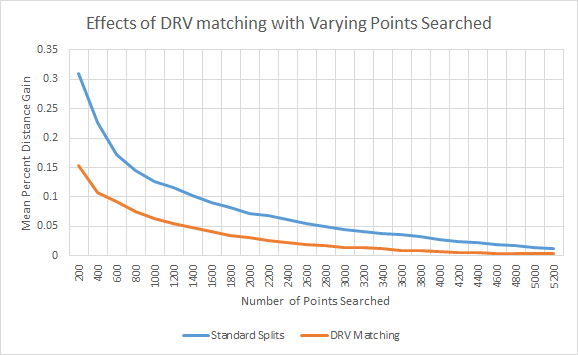
\includegraphics[width=\textwidth]{Figures/sysdesc_drv_varying_points}
\end{center}
\caption{Effects of DRV matching in a single k-d tree using SMS/WSMS with varying number of points searched}
\label{fig:drv_varying_points}
\end{figure}

\subsection{Tree Quality Metric}

While SPM and WSMS can result in greatly improved ANN performance, these methods are not directly feasible in practice on a system which supports specifying a DRV at query time rather than during tree construction.  As shown in Section \ref{subsec:const} the cost of generating a k-d tree is Nlog(N), while the cost of a standard linear query is N.  Thus, generating new trees to directly match the DRV of each query is not practical, as the tree construction cost is higher than a that of a linear search.

To work around this, we opted to construct a large set of k-d trees from a variety of different seed DRVs, whose selection process is detailed in Section \ref{sec:myalgconst}.  On receiving a query, our system can then select the tree or subset of trees whose seed DRVs best match the query's DRV.  In doing so, the set of trees searched will have been generated based on DRVs similar to that of the query, leading to improved performance for ANN queries.

The quality metric of a tree used is the modified Euclidean distance metric from equation \ref{eq:eucmod}.  Rather than comparing two points however, the two entities compared are the query DRV and the seed DRV of a tree, both of which have been normalized to have a sum of one.  The set of trees with the highest quality (smallest distance) can then be searched in parallel.  Additionally, based on the result of this tree quality metric, the parallel search between multiple trees can be skewed towards the trees of highest quality, searching these trees more deeply.

There is of course a tradeoff between the size of the set of k-d trees, and system performance.  More trees will result in high quality matches for more DRVs, and thus improved accuracy.  However, each additional tree is linear in memory consumption, so the number of these trees must be kept within reason.  Additionally, each test of the tree quality metric is computationally equivalent to a comparison between two points.  As such, the cost associated with computing the quality metric of each tree must be accounted for in performance benchmarks.

\section{Detailed Implementation Overview}
\label{sec:myimpl}

\subsection{Index Construction}
\label{sec:myalgconst}

The initial dataset input to the system is an unordered set of N points containing D dimensions.  The first step is to normalize all points in this set along each dimension using the scheme specified in Equation \ref{eq:normd} or \ref{eq:normd2}, per selection of the user.  The user must also select their split dimension heuristic to be SPM or WSMS as described in Section \ref{section:splitdim}.  Both heuristics are evaluated in Chapter \ref{results}.

The user also needs specify two index size parameters: the deterministic dimension depth (DDD) which will be explained shortly, and the number of random trees.  Both of these parameters impact the number of trees which will be generated.  The use of the DDD allows the system to perform well on DRVs which put very heavy weight on a low number of dimensions, which is likely to be common in practice.  To do so, a tree is generated with every possible subset of dimensions containing less than or equal to the DDD.  For each of these subsets, the seed DRV has equal weight in each of these dimensions, and as such are equivalent to $1/D$.  The number of trees needed to satisfy a DDD of R on a dataset with dimensionality D is shown in Equation \ref{eq:ddd}.  This number scales factorially with both D and R, so a very small R must be used if D is large to ensure that the number of trees is reasonable.  A large R however has the advantage of high quality tree matches on queries with R or less dimensions.

\begin{equation}
\label{eq:ddd}
ntrees = \sum\limits_{i=1}^R {D \choose i}
\end{equation}

The second parameter specifies the number of random trees using all dimensions, generated in addition to those based on the DDD parameter.  The number of random trees directly controls the number of trees generated with seed DRVS pulled from a uniform distribution.  Each initial weight on each dimension is a number selected randomly from U(0,1) on each dimension, and the results are normalized to have a sum of one.  A larger number of random trees will result in overall better matches on randomly selected DRVs at the cost of memory consumption.  Other types of dimension split priors other than uniform could be used instead if additional information was known about the distribution of DRVs used.  This possiblity is further considered in Chapter \ref{conclusion}

A final tree is also added which is seeded from a uniform DRV to perform standard ANN queries.  The total number of trees generated is thus the number of deterministic trees as specified by Equation \ref{eq:ddd} added with the number of random trees plus one.  Each tree is generated following the algorithm in Section \ref{subsec:const} with the modification that the split dimension is selected via SPM or WSMS rather than from a uniform distribution.  Implementation details about weighted random number selection are described in Section \ref{sec:rng}.  In our test environment, if the number of trees exceeds that which can be held in memory, they will be written to disk.  In practice, this would not be an acceptable solution, as the cost of reading a tree from memory is linear, and disk reads are significantly slower than a linear seek performed in memory \citep{ousterhout1989beating}.  Our evaluation metric, however, considers only the quality of results against the number of nodes searched, so this solution is acceptable for benchmarking purposes.  Details about implementation in a live, distributed system will be discussed in Chapter \ref{conclusion}.

The last step of construction after each tree is generated is to generate an index on the seed DRVs.  Without an index, in order to determine the best tree(s) for each query a linear seek across each seed DRV would need to be performed.  This would add an overhead of one comparison operation for each tree on every single ANN query.  To avoid this overhead, the seed DRVS are cast into a vector space.  After doing so, a k-d tree index is constructed on the seed DRVs following the standard procedure in section \ref{subsec:const}.  At query time, this index can be applied to heuristically select the best set of trees via an ANN search against the DRV in sublinear time.

\subsection{ANN Query}

Each ANN query requires a query point, a DRV, the number of results to return (K), and the maximum number of nodes to search (S).  Additional parameters shown in Table \ref{table:annparam} can also be optionally supplied to tune the search.  The first step of the algorithm, is to determine the top M trees to be used in the search.  Using the k-d tree index on the seed DRVs described in Section \ref{sec:myalgconst}, an ANN search is performed to determine these M trees and their respective quality scores against the DRV.  By default M is set to 3, and $.4 \times {total\_trees}$ nodes are searched.  However, both of these parameters can be adjusted.  For example, by setting the percentage of trees to search to 1, a linear search is performed instead.  Doing so is recommended for cases in which the dataset is large and the additional overhead from the linear search across all seed DRVs is negligible.

Since the initial quality metric is the distance between the query DRV and seed DRVs, a lower result of this metric represents a higher quality tree.  To obtain a quality metric in which a larger value represents high quality, $1/(distance + \epsilon)$ is used instead.  Epsilon was set as $10^{-10}$ to avoid a division by zero error on perfect matches while having minimal effect on the metric.  After M trees and their qualities are obtained, the qualities are normalized to have a sum of one.

Optionally, a tree pruning heuristic can be applied to remove trees of low quality in this set.  This is advantageous for queries with a low number of dimensions in the query DRV, as some trees in the top M may be of significantly high quality than others.  All trees with a normalized quality of less than $TC\times(1/M)$ are removed, where TC is the tree cutoff limit.  By default TC is set to .5 but a value of 0 results in the heuristic not being applied, as no trees will pass this check.  This heursitic has the additional benefit of reducing the set down to a single tree if a perfect or near perfect match is present.  If a distance is extremely close to zero, the quality metric for that tree will be extremely high, and after normalization will push that of other trees towards zero.  After trees are pruned, the qualities are re-normalized to a sum of one.

\begin{table}
\centering
\begin{tabular}{ | l | c | l |}
	\hline
	Optional Parameter & Default Value & Description \\
	\hline
	M & 5 & Maximum number of trees to search \\
	\hline
	SPS & $.1 \times$ number of trees & Seed DRVs to search \\
	\hline
	TC & .5 & Tree cutoff limit \\ 
	\hline
\end{tabular}
\caption{Optional Parameters}
\label{table:annparam}
\end{table}

Since the cost of comparing the DRV against a set of split probabilities is equivalent to that of searching a point, the number of seed DRVs checked is subtracted from S for the next part of the query.  The remaining searches are split among the selected trees proportional to the quality score of each tree.  In our testbed, the parallel search of these trees was emulated by a master thread switching between the search of each tree.  As mentioned in Section \ref{sec:randomforest}, the same priority queue was used during this search.  Additionally, a hash table was used on the id (a unique integer) of each point.  After a point was checked in one of the trees, the id was added to the hash table.  Upon checking the hash table in constant average time, the index can determine whether or not a point has been checked, and can avoid rechecking it if so.

The mechanisim for switching between between threads in our testbed is based on a single master.  At the start of an ANN query, M trees and their qualities are known.  A search is started on each tree in parallel; however, upon entering the critical area where a point would be searched the thread is put to sleep.  Using the algorithm described in Section \ref{sec:rng}, a random tree is selected with probabilities proporitional to each tree's quality.  This tree's thread is awakened, a single point is checked, and the thread is put back to sleep the next time it reaches the critical region.  When the maximum number of searches is reached, the master forces the search thread on each tree to return.  When all threads have returned, the top K will reside in the max priority queue shared between the threads.  Thus, with this method, the effect of searching the trees in parallel is emulated.  Implementation considerations for a true parallel or distributed implementation are discussed in Chapter \ref{conclusion}.

\subsection{Weighted Random Number Selection}
\label{sec:rng}

At multiple points in our system, weighted random number selection along D dimensions is performed, and as such it was important for the implementation to be efficient.  Given D weights normalized to a sum of one, these weights represent a probability distribution function (PDF) of each dimension being selected.  By summing these PDFs, a cumulative distribution function (CDF) was generated containing the probability of a dimension of d or less being selected.  To select a random dimension, a random double is drawn from a pseudorandom number generator uniformly distributed between zero and one.  A binary search is performed to determine the largest entry in the CDF which is greater than or equal to the selected number.  Thus, this implementation requires O(D) additional memory, O(D) preprocessing, and O(log(D)) time after each random number generation.